% Information:
% This is the Latex Slide Template for the ISA 419 Class
% Created by: Fadel Megahed | Email: fmegahed@miamioh.edu


%___________________________Initilization________________________________
% Other Colors/Themese can be found at: https://www.hartwork.org/beamer-theme-matrix/

% A] Notes or Presentation Mode
% Presentation
\documentclass[aspectratio=169]{beamer} % For Presentation Mode - see http://tex.stackexchange.com/questions/286366/how-to-increase-the-width-of-a-page-to-fit-the-fullscreen-mode-of-pdf
% [A] Theme Stuff
\usetheme{CambridgeUS}
\usecolortheme{beaver}
\definecolor{miamired}{RGB}{200,16,46}
\definecolor{darkgreen}{rgb}{0.09, 0.45, 0.27}
\definecolor{links}{HTML}{2A1B81}
\hypersetup{colorlinks,linkcolor=,urlcolor=links}
%\setbeamertemplate{footline}[frame number]
\setbeamercolor{title}{fg=miamired}
\setbeamercolor{block title}{bg=gray!35,fg=black}
\setbeamercolor{block body}{bg=gray!0,fg=black}
\setbeamercolor{frametitle}{fg=miamired}
\usefonttheme[]{serif}
\setbeamertemplate{items}[ball]
\setbeamercolor{alerted text}{fg=miamired,bg=}
\setbeamercolor*{item}{fg=miamired}
\setbeamercolor{section number projected}{bg=miamired}
\setbeamercolor{colorbox}{bg=miamired, fg=white}
\setbeamercolor{section in head/foot}{bg=miamired}
\setbeamercolor{author in head/foot}{bg=miamired}
\setbeamercolor{bibliography entry author}{fg=miamired}
\setbeamercolor{bibliography entry title}{fg=black} 
\setbeamercolor{bibliography entry location}{fg=miamired} 
\setbeamercolor{bibliography entry note}{fg=black!85}
\setbeamertemplate{bibliography item}[text]
%\setbeamertemplate{bibliography item}[article] % To have an article instead of the number
% https://tex.stackexchange.com/questions/183052/what-are-all-the-possible-first-arguments-to-setbeamerfont/183053#183053
\setbeamerfont{alerted text}{series=\bfseries}
\setbeamerfont{block title}{series=\bfseries}
\setbeamerfont{block body}{series=\bfseries}
\setbeamerfont{itemize item}{series=\bfseries}
\setbeamerfont*{itemize/enumerate subbody}{parent=itemize/enumerate body}
\setbeamerfont*{itemize/enumerate subsubbody}{parent=itemize/enumerate body}
\setbeamerfont{section in toc}{series=\bfseries}
\setbeamerfont{frametitle}{series=\bfseries}
\setbeamerfont{footline}{series=\tiny}
\setbeamerfont{headlineline}{series=\tiny}
\setbeamerfont{section in head/foot}{series=\tiny}
\setbeamerfont{subsection in head/foot}{series=\tiny}
\setbeamerfont{subsubsection in head/foot}{series=\tiny}
\setbeamerfont{page number in head/foot}{series=\tiny}
\setbeamerfont{date}{series=\scriptsize}
\setbeamerfont{date in head/foot}{series=\tiny}
\setbeamercolor*{block title example}{fg=miamired,
	bg=miamired!10}
\setbeamercolor*{block body example}{fg= black}

\setbeamerfont{bibliography item}{size=\footnotesize}
\setbeamerfont{bibliography entry author}{size=\footnotesize}
\setbeamerfont{bibliography entry title}{size=\footnotesize}
\setbeamerfont{bibliography entry location}{size=\footnotesize}
\setbeamerfont{bibliography entry note}{size=\footnotesize}

% [B] Needed Packages
\usepackage[export]{adjustbox}
\usepackage{amsfonts}
\usepackage{amsmath}
\usepackage{amssymb}
\usepackage{animate}
\usepackage{array}
\newcolumntype{m}[1]{>{\arraybackslash\hspace{0pt}}p{#1}}
\usepackage[justification=centering]{caption}
\usepackage{colortbl}
\usepackage{etoolbox}
\usepackage{fancybox}
\usepackage{fontawesome5}
\usepackage{framed}
\usepackage{graphics}
\usepackage{graphicx}
\usepackage{hyperref} 
\usepackage[utf8]{inputenc}
\usepackage{makecell}
\usepackage{mathtools}
\usepackage{marvosym}
\usepackage[framemethod=default]{mdframed}
\usepackage{media9}
%\addmediapath{./Figures/}
\usepackage{multicol}
%\usepackage{multimedia}
\usepackage{multirow}
\usepackage{pgfplots} %for tikzpictures
\usepackage{sidecap}
\usepackage{smartdiagram}
\usepackage{soul}
\usepackage{subfigure}
\usepackage{tikz}
\usetikzlibrary{shapes.geometric, arrows}
\usepackage{times}
\usepackage{url}
	\urlstyle{same}
\usepackage{wasysym} % for smiley faces
\usepackage{wrapfig}








% [C] New Commands and Default Pathes
\newcommand{\EndofPage}{\vskip0pt plus 1filll}
\newcommand{\norm}[1]{\left\lVert#1\right\rVert}
\graphicspath{ {../../figures/} }
\setbeamertemplate{frametitle continuation}{[\insertcontinuationcount]}
\setbeamercovered{still covered={\opaqueness<1->{5}},again covered={\opaqueness<1->{60}}}
% begining of the new definition
\makeatletter
\newcommand*\fix@beamer@close{%
	\ifnum\beamer@trivlistdepth>0
	\beamer@closeitem
	\fi
}
\newcommand*\fix@beamer@open{%
	\ifnum\beamer@trivlistdepth>0
	\gdef\beamer@closeitem{}%
	\fi
}
\BeforeBeginEnvironment{itemize}{\fix@beamer@close}
\AfterEndEnvironment{itemize}{\fix@beamer@open}
\makeatother
% end of the new definition

% For Boxes
\newmdenv[skipabove=7pt,
skipbelow=7pt,
rightline=false,
leftline=true,
topline=false,
bottomline=false,
backgroundcolor= miamired!10,
linecolor= miamired,
innerleftmargin=5pt,
innerrightmargin=5pt,
innertopmargin=5pt,
innerbottommargin=5pt,
leftmargin=0cm,
rightmargin=0cm,
linewidth=4pt]{eBox}

\newmdenv[skipabove=7pt,
skipbelow=7pt,
rightline=false,
leftline=true,
topline=false,
bottomline=false,
linecolor=miamired,
innerleftmargin=5pt,
innerrightmargin=5pt,
innertopmargin=0pt,
leftmargin=0cm,
rightmargin=0cm,
linewidth=4pt,
innerbottommargin=0pt]{dBox}

\newtheorem{exampleT}{Example}[section]
\newenvironment{ExamplesT}{\begin{exampleT}}{\hfill{\tiny\ensuremath{\blacksquare}}\end{exampleT}}


\newenvironment{conditions}
{\par\vspace{\abovedisplayskip}\noindent\begin{tabular}{>{$}l<{$} @{${}={}$} l}}
	{\end{tabular}\par\vspace{\belowdisplayskip}}
%%%%%%%%%%%%%%%%%%%%%%%%%%%%%%%%%%%%%%%%%%%%%%%%%%%%%%%%%%%%%%


\AtBeginSection[]
{
	\begin{frame}{Outline}
	\tableofcontents[currentsection, %subsectionstyle=show/shaded/hide,
	subsectionstyle=hide,
	subsubsectionstyle=hide]
\end{frame}
}

\AtBeginSubsection[]
{
\begin{frame}{Outline}
\tableofcontents[currentsection, %subsectionstyle=show/shaded/hide, %subsubsectionstyle=hide]
\end{frame}
}
\mode<beamer>

%____________________ Title, Author, Affliation & Date____________________
\title{ISA 419: Data Driven Security}
\subtitle{}
\author{Fadel M. Megahed}

\institute[Miami University]{
	Endres Associate Professor\\
	Department of Information Systems and Analytics \\
	Farmer School of Business \\ 
	Miami University \\
	\faPaperPlane \ \href{mailto:fmegahed@miamioh.edu?subject=ISA 419 Questions}{fmegahed@miamioh.edu} \\
	\faQuestion \ \href{https://calendly.com/fmegahed/}{by appointment} @ 2004 FSB}

\date{Spring 2022} %\date{\scriptsize{\today}}
%%%%%%%%%%%%%%%%%%%%%%%%%%%%%%%%%%%%%%%%%%%%%%%%%%%%%%%%%%%%%%%%%%%%%%%%%%

\begin{document}
%______________________________________________________________________________	
%Frame 1
	\maketitle
	
% Frame 2
\begin{frame}
	\frametitle{\textbf{Learning Objectives for Today's Class}}
	\begin{block}{\textbf{Main Learning Outcomes for Today's Class}}
		\begin{itemize}
			\item \textbf{Define information security (infoSec), its main goals, and how it fits within a firm's overall security protocols}
			\item \textbf{Describe the three main steps in information security}
			\item \textbf{Explain why prevention as a sole security measure is deemed to fail}
			\item \textbf{Describe course objectives \& structure}
			\item \textbf{Assess your ability to explore a somewhat simple infoSec dataset}
		\end{itemize}
	\end{block}
\end{frame}

\section{An Overview of Cyber/Information Security}

% Frame 4
\begin{frame}{\textbf{What is security?}}
	\begin{block}{\textbf{Definition}}
		\begin{itemize}
			\item \textbf{According to the Merriam-Webster Dictionary \cite{mWebster2020sec}, security can be defined as: \textcolor{miamired}{``the quality or state of being secure: such as freedom from danger.''}}
			
			\item \textbf{In other words, the overall objective is to protect \textcolor{miamired}{against adversaries who would do harm whether it is intentional or not} \cite{whitman2011principles}.}
			
			\item \textbf{For example, \ul{national security} is a \textcolor{miamired}{``multilayered system that protects the sovereignty of a state, its assets, its resources, and its people.''} \cite[p. 8]{whitman2011principles}}
		\end{itemize}
		
	\end{block}
\end{frame}

% Frame 5
\begin{frame}{\textbf{What is security? A firm's perspective}}
	\centering 
	
	\smartdiagramset{
		uniform color list= miamired for 4 items,
		bubble node size = 2.25cm,
		bubble center node size = 3.33 cm,
		bubble center node font = \small,
		bubble node font = \small
	}
	
	\smartdiagram[bubble diagram]{
		\textbf{Firm's} \\ \textbf{Security} \\ \textbf{Dimensions},\textbf{ Physical}, \textbf{Personnel}, \textbf{Operations}, \textbf{Network}, \textbf{Information}}	
	
	% See P.8 in Principles of Information Security
\end{frame}

% Frame 6
\begin{frame}{\textbf{What is cyber/information security?}}
	\textbf{While some researchers distinguish between them \cite{von2013information}, in this course, we will use both terms \textcolor{miamired}{interchangeably}. Possible \textcolor{miamired}{definitions for cyber/information security include:}}

	\begin{block}{\textbf{Definition}}
		\begin{itemize}
			\item \textbf{According to the Merriam-Webster Dictionary \cite{mWebster2020cybersec}, cyber security can be defined as: \textcolor{miamired}{``measures taken to protect a computer or computer system (as on the Internet) against unauthorized access or attack''}}
			
				
			\item \textbf{According to the SANS Institute \cite{sans2020infosec},  \textcolor{miamired}{``information security refers to the processes and methodologies which are designed and implemented to protect print, electronic, or any other form of confidential, private and sensitive information or data from \ul{unauthorized access}, \ul{use}, \ul{misuse}, \ul{disclosure}, \ul{destruction}, \ul{modification}, or \ul{disruption}.''}}
		\end{itemize}
		
	\end{block}
\end{frame}

% Frame 7
\begin{frame}{\textbf{Information Security Goals: CIA [1]}}
	\begin{block}{\textbf{Confidentiality, Integrity, and Availability (CIA)}}
		\begin{itemize}
			\item \textbf{\textcolor{miamired}{Confidentiality:} Preventing unauthorized reading/disclosure of information.}
			
			\item \textbf{\textcolor{miamired}{Integrity:} Preventing unauthorized modification of information.}
			
			\item \textbf{\textcolor{miamired}{Availability:} Preventing unauthorized withholding of information/ resources.}
		\end{itemize}
	\end{block}
\end{frame}

% Frame 8
\begin{frame}{\textbf{Information Security Goals: CIA [2]}}
	\textbf{Suppose that I would like to start an online banking business, named Miami University Online Bank (MUOB). Assume that we have:}
	
	\begin{figure}[!htb] 
		\minipage{0.32\textwidth}
		\centering
		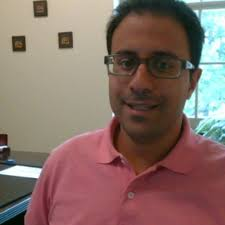
\includegraphics[width=\linewidth, height=2.5cm, keepaspectratio]{fmegahed.jpg}
		\caption{Fadel (Owner)}\label{fig:fadel}
		\endminipage\hfill
		\minipage{0.32\textwidth}
		\centering
		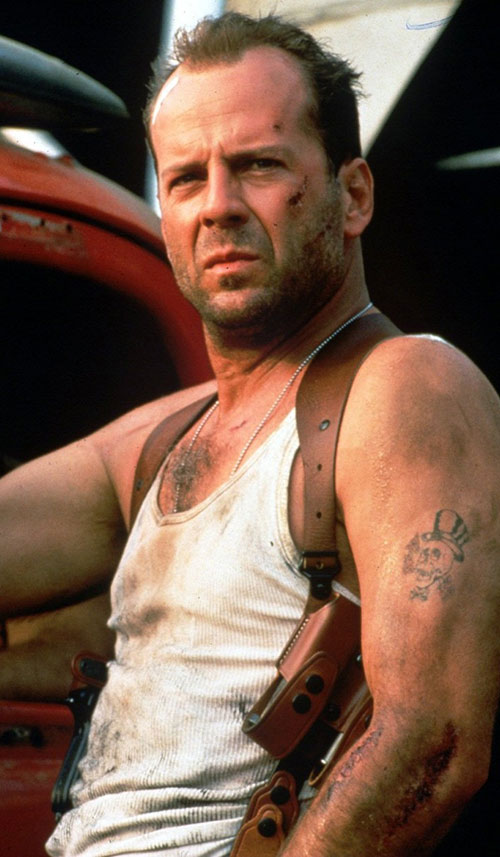
\includegraphics[width=\linewidth, height=2.5cm, keepaspectratio]{john.jpg}
		\caption{John (Customer)}\label{fig:john}
		\endminipage\hfill
		\minipage{0.32\textwidth}%
		\centering
		
\includegraphics[width=\linewidth, height=2.5cm, keepaspectratio]{hans.png}
		\caption{Hans (Bad Guy)}\label{fig:hans}
		\endminipage
	\end{figure}
	
	\textbf{\textcolor{miamired}{Question: How can you explain to me the CIA principles in the context of MUOB?}}
	% see Section 1.2.1 in https://www.google.com/books/edition/Information_Security/UW3SS9P9hdEC?hl=en&gbpv=1&printsec=frontcover
\end{frame}

% Frame 9
\begin{frame}{\textbf{Information Security Goals: Beyond the CIA Principles}}
	\centering 
	\smartdiagramset{
		uniform color list= miamired for 5 items,
		bubble node size = 2.25cm,
		bubble center node size = 3.33 cm,
		bubble center node font = \small,
		bubble node font = \small
	}
	
	\smartdiagram[bubble diagram]{
		\textbf{Beyond} \\ \textbf{the} \textbf{CIA},\textbf{ Authentication} \\ (computer \\ vs. network), \textbf{Authorization}, \textbf{Privacy}, \textbf{Non-repudiation}, \textbf{Auditability}}	
\end{frame}

% Frame 10
\begin{frame}{\textbf{A Taxonomy of Information Security (Defense) Measures}}
	\centering
	
	\vspace{\baselineskip}
	
	\smartdiagramset{
		uniform color list= miamired for 3 items, 
		module minimum width = 3.5 cm,
		text width= 3 cm,
		font = \normalfont, 
		circular distance = 2.5 cm,
		uniform arrow color = true, 
		arrow color = gray
	}
	
	\smartdiagram[circular diagram:clockwise]{\textbf{Prevention}, \textbf{Detection}, \textbf{Response}}
	
	\EndofPage
	
	\scriptsize{\textbf{Source:} Adapted from CS 259D, Stanford University, \url{https://web.stanford.edu/class/cs259d/lectures/Session1.pdf}}
	
	\vspace{0.5\baselineskip}
\end{frame}

% Frame 11
\begin{frame}{\textbf{Risk Management Controls as Preliminary Preventive Measures}}
	
	\vspace{\baselineskip}
	
	\begin{block}{\textbf{Risk Management Controls}}
		\begin{itemize}
			\item<1-3> \textbf{\textcolor{miamired}{Administrative:} Includes the development and deployment of policies and procedures; for example:}
			\begin{itemize}
				\item<2> \textbf{Password policies}
				\item<3> \textbf{Principal of least privilege (POLP)}
			\end{itemize}
			
			\item<4> \textbf{\textcolor{miamired}{Physical:} In addition to securing a firm's premises through doors/locks/etc., typical risk management controls utilize the:}
			\begin{itemize}
				\item<4> \textbf{Principal of separation of duties}
			\end{itemize} 
		\end{itemize}
	\end{block}
	
	\EndofPage
	
	\centering \scriptsize{\textbf{Source:} Adapted from CS 259D, Stanford University, \url{https://web.stanford.edu/class/cs259d/lectures/Session1.pdf}}
	
	\vspace{0.5\baselineskip}
\end{frame}

% Frame 12
\begin{frame}{\textbf{Other Preventive Measures}}
	
	\vspace{\baselineskip}
	
	\begin{block}{\textbf{Other Important Preventive Measures}}
		\begin{itemize}
			\item \textbf{\textcolor{miamired}{Protocols:} For example, the reliance on secure socket layer (SSL) to authenticate the web source}
			
			\item \textbf{\textcolor{miamired}{Host-based protections:} secure operating systems and/or patching}
			
			\item \textbf{\textcolor{miamired}{Access Control:} Through identification (username), authentication (over a computer/ network), and authorization (file permissions, need-to-know principle)}
			
			\item \textbf{\textcolor{miamired}{Firewalls:} to control inter-network traffic (e.g., from/to internet)}
			
			\item \textbf{\textcolor{miamired}{Security by design:} code reviews, unit testing, defense in depth, and principle of least privilege}
		\end{itemize}
	\end{block}

	\EndofPage

	\centering \scriptsize{\textbf{Source:} Adapted from CS 259D, Stanford University, \url{https://web.stanford.edu/class/cs259d/lectures/Session1.pdf}}
	
	\vspace{0.5\baselineskip}
\end{frame}

% Frame 13
\begin{frame}{Failure of Prevention: Attacking Constantly Getting Easier}
	\centering 
	
	\vspace{0.25\baselineskip}
	
	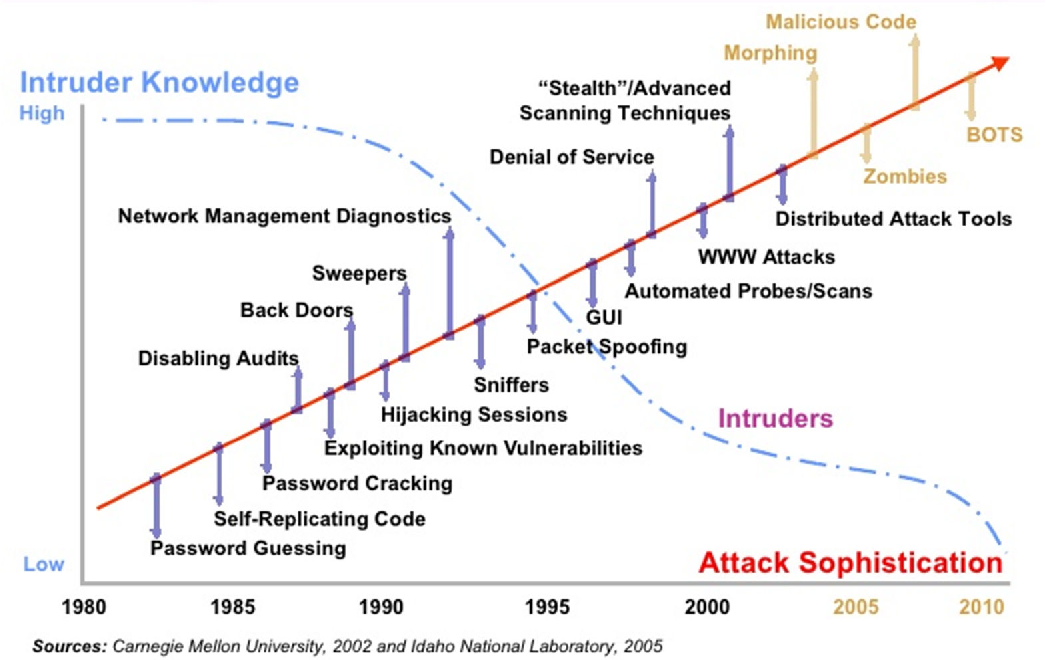
\includegraphics[width=\linewidth, height = 0.75\textheight, keepaspectratio, frame]{attack-soph.png}
	
	\EndofPage
	
	\centering \scriptsize{\textbf{Source:} Figure 1-1 in  Pacheco Ramirez's PhD Dissertation \cite{pacheco2017anomaly}, University of Arizona.}
	
	\vspace{0.5\baselineskip}
\end{frame}

% Frame 14
\begin{frame}{Failure of Prevention: Attacking Constantly Getting Faster}
	\centering 
	
	\vspace{0.25\baselineskip}
	
	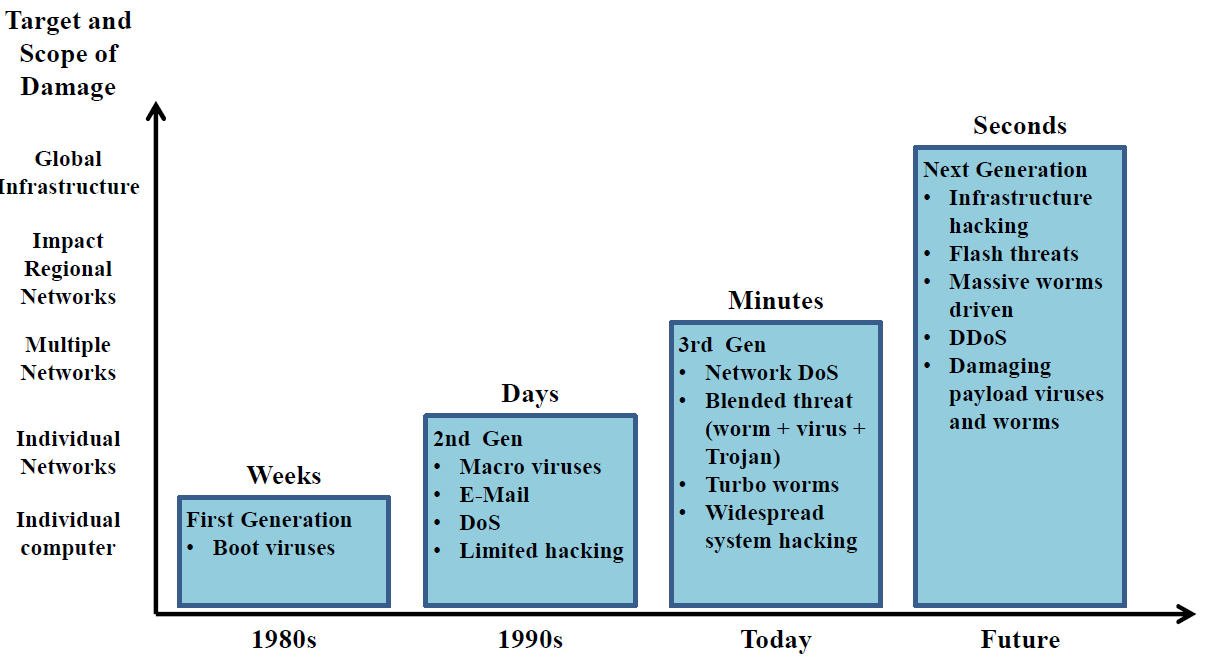
\includegraphics[width=\linewidth, height = 0.75\textheight, keepaspectratio, frame]{attack-time.PNG}
	
	\EndofPage
	
	\centering \scriptsize{\textbf{Source:} Figure 1-2 in Pacheco Ramirez's PhD Dissertation \cite{pacheco2017anomaly}, University of Arizona.}
	
	\vspace{0.5\baselineskip}
\end{frame}

% Frame 15
\begin{frame}{Failure of Prevention: Attackers Having More Options due to IoT}
	\centering 
	
	\vspace{0.25\baselineskip}
	
	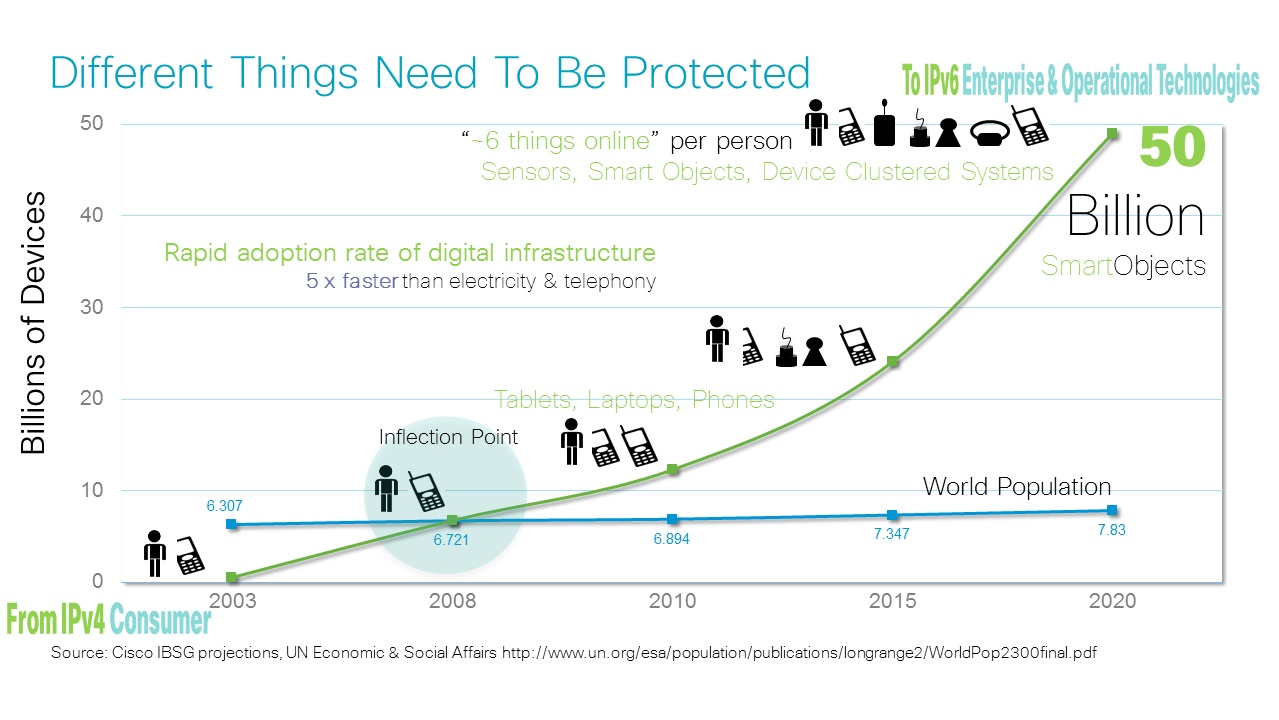
\includegraphics[width=\linewidth, height = 0.75\textheight, keepaspectratio, frame]{iot-figure1.jpg}
	
	\EndofPage
	
	\centering \scriptsize{\textbf{Source:} Figure 1 in Cisco's \textit{Securing the Internet of Things: A Proposed Framework} \cite{pacheco2017anomaly}.}
	
	\vspace{0.5\baselineskip}
\end{frame}

% Frame 16
\begin{frame}{\textbf{Failure of Prevention: Possible Root-Causes}}
		\begin{columns}
			\begin{column}{0.6\textwidth}
				\begin{block}{\textbf{Inherent weaknesses in increasingly complex systems}}
					\begin{itemize}
						\item \textbf{Poor design} affecting software and hardware
						\item \textbf{Poor implementation} due to security being an afterthought, lack of personnel experience, \& poor system configuration
						\item \textbf{Poor management}, i.e. inadequate policies/ procedures
						\item \textbf{Trade-offs} between security and usability
						\item \textbf{Humans} using computer/network systems; \textcolor{miamired}{\textbf{We are the weakest link in any system}}  
					\end{itemize}
				\end{block}
			\end{column}
			\begin{column}{0.35\textwidth}
				\begin{block}{\textbf{Vulnerabilities}}
					\begin{itemize}
						\item \textbf{Back doors}
						\item \textbf{Denial of Service}
						\item \textbf{Exploits}
						\item \textbf{Social engineering}
					\end{itemize}
				\end{block}
			\end{column}
		\end{columns}

	\EndofPage
	
	\centering \scriptsize{\textbf{Source:} Adapted from CS 259D, Stanford University, \url{https://web.stanford.edu/class/cs259d/lectures/Session1.pdf}}
	
	\vspace{0.5\baselineskip}

\end{frame}

% Frame 17
\begin{frame}{Class Activity: Failure of Prevention - Have you been pwned?}
	\textbf{The purpose of this class activity is to investigate how many of your web accounts have been breached. This activity consists of the following steps:}
	
	\begin{itemize}
		\item \textbf{Go to: \textcolor{miamired}{\url{https://haveibeenpwned.com/}}}
		
		\item \textbf{Insert the email you use most online (e.g., in my case it is my gmail) into the search bar and then click on ``pwned?''}
		
		\item \textbf{Record the number of breaches that you were pwned in, using the code shown in class for the website: \textcolor{miamired}{\url{www.menti.com}}}
		
		\item \textbf{\textcolor{gray}{Outside of class: Address the breaches by changing your password for these sites, opting into 2-factor authentication, and changing the passwords in other websites (if you re-used this password).}}
	\end{itemize}
\end{frame}

% Frame 18
\begin{frame}{Failure of Prevention: World's Biggest Data Breaches \& Hacks}
	\centering
	
	\href{https://www.informationisbeautiful.net/visualizations/worlds-biggest-data-breaches-hacks/}{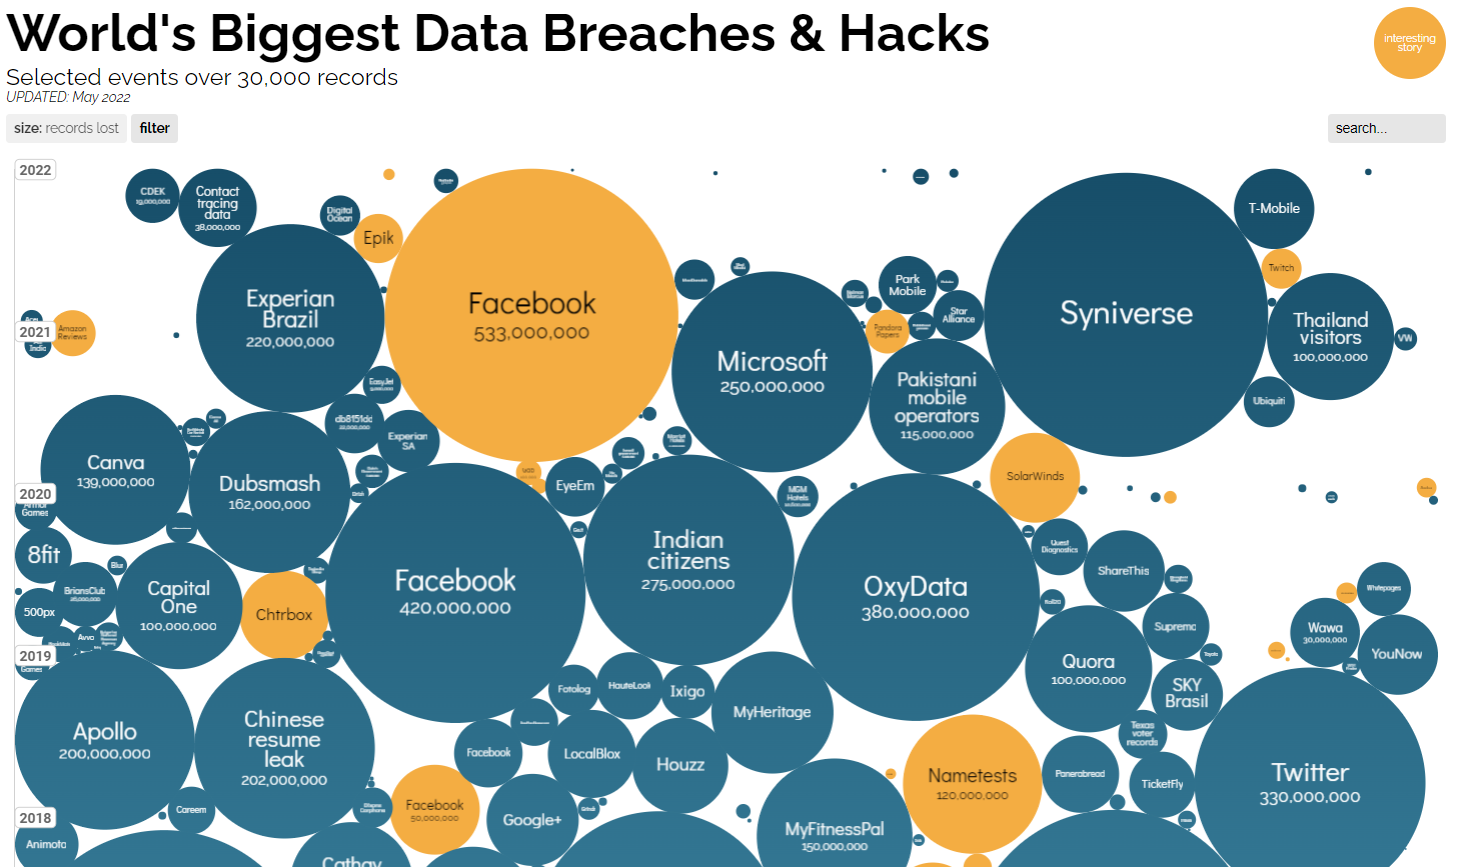
\includegraphics[width=\textwidth, height=0.8\textheight, keepaspectratio, frame]{data-breaches.PNG}}
	
		\EndofPage
	
	\centering \scriptsize{\textbf{Source:} \url{https://www.informationisbeautiful.net/visualizations/worlds-biggest-data-breaches-hacks/}}
	
	\vspace{0.5\baselineskip}
\end{frame}

% Frame 19
\begin{frame}{Failure of Prevention: Most Targeted Industries}
	\centering
	
	\href{https://www.nasdaq.com/articles/cybersecurity-industry-report-investment-case-2018-06-25}{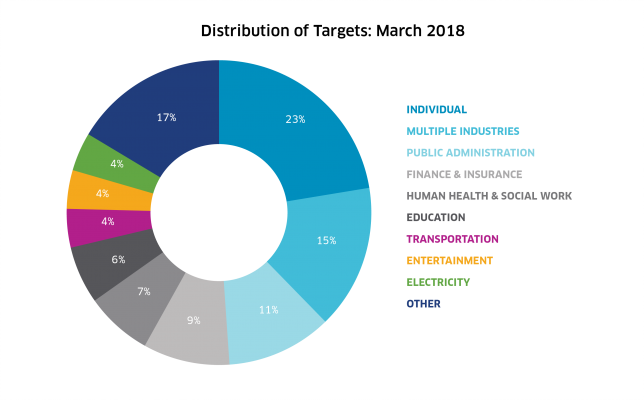
\includegraphics[width=\textwidth, height=0.8\textheight, keepaspectratio, frame]{nasdaq-targets.png}}
	
	\EndofPage
	
	\centering \scriptsize{\textbf{Source:} \url{https://www.nasdaq.com/articles/cybersecurity-industry-report-investment-case-2018-06-25}}
	
	\vspace{0.5\baselineskip}
\end{frame}

% Frame 20
\begin{frame}{Detective Security [1]}
	\begin{dBox}
		\begin{quotation}
			\noindent \textbf{Detection of a system compromise is extremely critical. With the ever increasing threat environment, no matter what level of protection a system may have, it will get compromised given a greater level of motivation and skill. There is no full proof ``silver bullet'' security solution. \textcolor{miamired}{A defense in layers strategy should be deployed so when each layer fails, it fails safely to a known state and sounds an alarm.} The most important element of this strategy is \textcolor{miamired}{timely detection and notification of a compromise}. Intrusion detection systems (IDS) are utilized for this purpose. } \textbf{Sans Institute \cite[p. 4]{sans2002info}}
		\end{quotation}
	\end{dBox}

	\EndofPage
	
	\centering \scriptsize{\textbf{Note:} You are expected to read P. 1-6 in \cite{sans2002info}. Refer to the References Slides for detailed information.}
	
	\vspace{0.5\baselineskip}
		
\end{frame}

% Frame 21
\begin{frame}{Detective Security [2]}
	\begin{dBox}
		\begin{quotation}
			\noindent \textbf{As previously indicated, intrusion detection is much more than an alarm. Although it is an alarm, it's an \textcolor{miamired}{alarm with brains}. Imagine a fire alarm that had the capability of detecting a fire, distinguish the type of fire, pinpoint its source and path, alert the building
			occupants and fire department, and forward intelligence to the firehouse prior to their response. All this and even having the capability of distinguishing normal activity such as bad cooking. A properly configured intrusion detection system is such a device. An alarm with brains.} \textbf{Sans Institute \cite[p. 4]{sans2002info}}
		\end{quotation}
	\end{dBox}
	
	\EndofPage
	
	\centering \scriptsize{\textbf{Note:} You are expected to read P. 1-6 in \cite{sans2002info}. Refer to the References Slides for detailed information.}
	
	\vspace{0.5\baselineskip}
	
\end{frame}

% Frame 22
\begin{frame}{Response: What to do in case of detecting a security breach?}
	\textbf{There are two popular/similar frameworks for incident response:}
	\centering 
	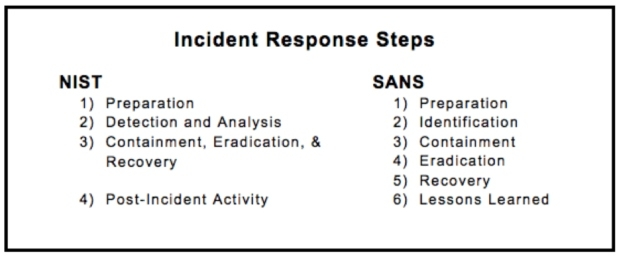
\includegraphics[width=0.7\textwidth]{incident-response-steps-comparison-guide-framework-side-by-side.jpg}
	
	\EndofPage
	
	\centering \scriptsize{\textbf{Source:} First figure in the AT\&T Cybersecurity blog post by Elisha Girken \cite{girken2020incident}.}
	
	\vspace{0.5\baselineskip}
\end{frame}

%---------------------------------------------------------------------------
\section{Course Expectations \& Overview}
% Frame 4
\begin{frame}{\textbf{Course Overview [1]}}
	\textbf{Traditionally, information technology (IT) security was a job that entailed using a few tools, solutions and best practices that focused on attack prevention and protect a company's sensitive information and network assets. However, these solutions are no longer sufficient. The businesses are transitioning to a new era, where cybersecurity is \textcolor{miamired}{enhanced and almost requires data-driven analytical solutions.} The primarily goals of data-driven security are to: (a) discover malicious patterns from the data-lakes of logs produced by security software, and (b) develop automated tools that can assist in the surveillance of security-related data. This course covers various analytic applications in information/cyber security including: \textcolor{miamired}{user behavior analysis, network and host intrusion detection, web security, phishing detection, and emerging issues in Industrial Internet of Things (IIoT) security.} Note that the course is designed to be \textcolor{miamired}{very applied, involving a large amount of programming to examine real datasets.}}
\end{frame}

% Frame 5
\begin{frame}{\textbf{Course Overview [2]}}
	\begin{figure}[h!]
		\centering
		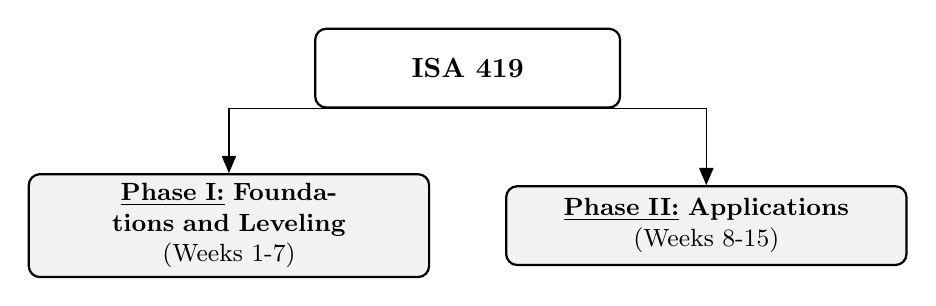
\begin{tikzpicture}[node distance=2cm, font=\small]
		\tikzstyle{start} = [rectangle, rounded corners, minimum width=0.3\textwidth, minimum height=1cm,text badly centered, text width=0.3\textwidth, draw=black, thick,font=\normalfont]
		
		\tikzstyle{categories} = [rectangle, rounded corners, minimum width=0.4\textwidth, minimum height=1cm,text centered, text width=0.4\textwidth, draw=black, fill=gray!10, thick]
		
		
		\tikzstyle{arrow} = [->,>= triangle 45]
		
		% Begining of the creation of the figure
		\node (start) [start] {\textbf{ISA 419}};
		
		% Level 1 nodes
		\node (ba) [categories, below of = start, xshift=-0.25\textwidth] {\textbf{\underline{Phase I:} Foundations and Leveling} \\ (Weeks 1-7)};
		\node (app) [categories, below of = start, xshift = 0.25\textwidth] {\textbf{\underline{Phase II:} Applications} \\ (Weeks 8-15)};	
		
		% Arrows
		\draw [arrow] (start.south) -| (ba);
		\draw [arrow] (start.south) -| (app);
	\end{tikzpicture}
	\caption{How the ISA 419 course is organized. See the \href{https://miamioh.instructure.com/courses/179824/pages/schedule}{tentative class schedule} for more details.}
	\end{figure}	
\end{frame}


% Frame 6
\begin{frame}{\textbf{Course Objectives}}
	\textbf{Upon completing the course, you will:}
	\begin{itemize}
		\item \textbf{Describe key cybersecurity concepts including the CIA Triad, access management, incident response and common cybersecurity best practices.}
		\item \textbf{Demonstrate a fundamental understanding of the role of analytical solutions in state-of-the-art cybersecurity solutions.}
		\item \textbf{Understand the uniqueness of cybersecurity datasets, including:  the nature of unbalanced data and diversity of data in each class, asymmetrical costs of misclassification and non-stationary inference.}
		\item \textbf{Have a basic understanding of the theory behind some commonly used statistical methodologies and machine learning algorithms in data-driven security.}
		\item \textbf{Use and implement an appropriate modeling paradigm to tackle cybersecurity problems.}
	\end{itemize}
\end{frame}


% Frame 7
\begin{frame}{\textbf{Instructional Approach}}
	\begin{figure}[h!]
		\centering
		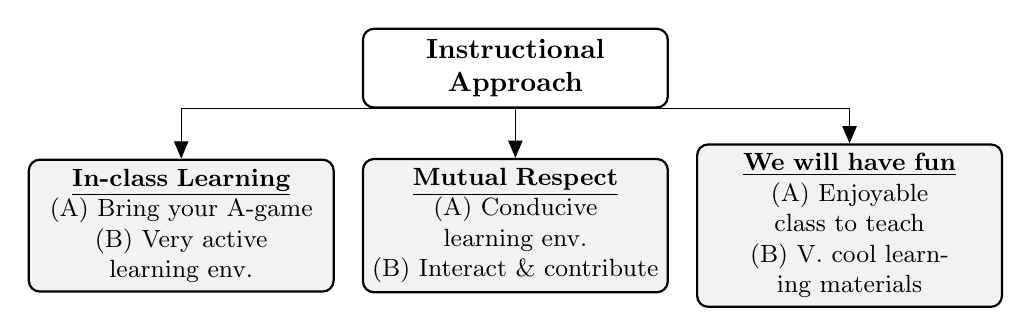
\begin{tikzpicture}[node distance=2cm, font=\small]
		\tikzstyle{start} = [rectangle, rounded corners, minimum width=0.3\textwidth, minimum height=1cm,text badly centered, text width=0.3\textwidth, draw=black, thick,font=\normalfont]
		
		\tikzstyle{categories} = [rectangle, rounded corners, minimum width=0.3\textwidth, minimum height=1cm,text centered, text width=0.3\textwidth, draw=black, fill=gray!10, thick]
		
		
		\tikzstyle{arrow} = [->,>= triangle 45]
		
		% Begining of the creation of the figure
		\node (start) [start] {\textbf{Instructional Approach}};
		
		% Level 1 nodes
		\node (ia1) [categories, below of = start, xshift=-0.35\textwidth] {\textbf{\underline{In-class Learning}} \\ (A) Bring your A-game \\ (B) Very active learning env.};
		\node (ia2) [categories, below of = start, xshift = 0in] {\textbf{\underline{Mutual Respect}} \\ (A) Conducive learning env. \\ (B) Interact \& contribute};	
		\node (ia3) [categories, below of = start, xshift=0.35\textwidth] {\textbf{\underline{We will have fun}} \\ (A) Enjoyable class to teach \\ (B) V. cool learning materials};
		
		% Arrows
		\draw [arrow] (start.south) -| (ia1);
		\draw [arrow] (start.south) -| (ia2);
		\draw [arrow] (start.south) -| (ia3);
		\end{tikzpicture}
		\caption{An overview of the instructional approach for ISA 419.}
	\end{figure}
\end{frame}

% Frame 8
\begin{frame}{\textbf{How will I Evaluate your Learning?}}
	\begin{figure}[h!]
		\centering
		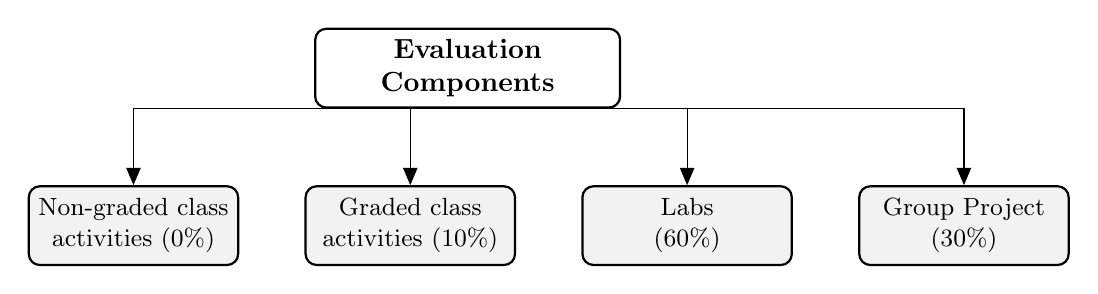
\begin{tikzpicture}[node distance=2cm, font=\small]
		\tikzstyle{start} = [rectangle, rounded corners, minimum width=0.3\textwidth, minimum height=1cm,text centered, text width=0.3\textwidth, draw=black, thick,font=\normalfont]
		
		\tikzstyle{categories} = [rectangle, rounded corners, minimum width=0.2\textwidth, minimum height=1cm,text centered, text width=0.2\textwidth, draw=black, fill=gray!10, thick]
		
		
		\tikzstyle{arrow} = [->,>= triangle 45]
		
		% Begining of the creation of the figure
		\node (start) [start] {\textbf{Evaluation Components}};
		
		% Level 1 nodes
		\node (e1) [categories, below of = start, xshift=-0.35\textwidth] {Non-graded class \\ activities (0\%)};
		\node (e2) [categories, right of = e1, xshift=0.125\textwidth] {Graded class \\ activities (10\%)};
		\node (e3) [categories, right of = e2, xshift=0.125\textwidth] {Labs \\ (60\%)};
		\node (e4) [categories, right of = e3, xshift=0.125\textwidth] {Group Project \\ (30\%)};
	
		% Arrows
		\draw [arrow] (start.south) -| (e1);
		\draw [arrow] (start.south) -| (e2);
		\draw [arrow] (start.south) -| (e3);
		\draw [arrow] (start.south) -| (e4);
		
		\end{tikzpicture}
		\caption{An overview of the evaluation components for ISA 419.}
	\end{figure}
\end{frame}


%-----------------------------------------------------------------
\section{Self-Assessment of Ability to Explore a Sample InfoSec Dataset}

% Frame
\begin{frame}{Activity: Explore the Los Alamos National Laboratory's Dataset}
	In 2014, researchers from the Los Alamos National Laboratory have made available a dataset on ``User-Computer Authentication Associations in Time''. A brief description of the dataset is available at: \url{https://csr.lanl.gov/data/auth/}. In this class activity, you are asked to examine a sample of the data, which can be downloaded from:
	\begin{itemize}
		\item \url{https://www.dropbox.com/s/88ajdyp7hfnvrl2/lanl-auth-dataset-1-03.csv} (where you will need to click on the triangle next to open to download the unzipped ``.csv'' file)
	\end{itemize} 
	
	\vspace{\baselineskip}
	
	\textbf{For the data in lines 1.1M-1.2M, please answer the following questions:}
	\begin{itemize}
		\item What is the timestamp of observation (i.e. row number) 1,200,000? % 
		\item What are the number of unique users for the aforementioned 100,000 observations?
		\item What is the number of unique computers used by U12 for the aforementioned 100,000 observations?
	\end{itemize}
\end{frame}

%-----------------------------------------------------------------------
\section{Recap and Things to Do}

% Frame
\begin{frame}{The FBI Director's Remarks in the RSA Security Conference}
	
	\begin{figure}
		\centering
		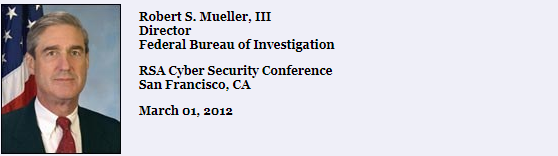
\includegraphics[width=0.75\textwidth]{mueller.PNG}
	\end{figure}
	
	\begin{quotation}
		\noindent ``\textbf{I am convinced that there are only two types of companies: those that have been hacked and those that will be. And even they are converging into one category: companies that have been hacked and will be hacked again.}''  
	\end{quotation}

	\vspace{0.75\baselineskip}

	\scriptsize{\textbf{Source:} \url{https://archives.fbi.gov/archives/news/speeches/combating-threats-in-the-cyber-world-outsmarting-terrorists-hackers-and-spies}}
\end{frame}

% Frame
\begin{frame}
	\frametitle{\textbf{Learning Objectives for Today's Class}}
	\begin{block}{\textbf{By the end of the class, you should be able to:}}
		\begin{itemize}
			\item \textbf{Define information security (infoSec), its main goals, and how it fits within a firm's overall security protocols}
			\item \textbf{Describe the three main steps in information security}
			\item \textbf{Explain why prevention as a sole security measure is deemed to fail}
			\item \textbf{Describe course objectives \& structure}
			\item \textbf{Assess your ability to explore a somewhat simple infoSec dataset}
		\end{itemize}
	\end{block}
\end{frame}

% Frame
\begin{frame}{Things to Do Before Next Class}
	\begin{block}{\textbf{Suggested Activities before Next Class}}
		\begin{itemize}
			\item \textbf{You should read the Sans Institute's Information Security Process \cite{sans2002info}.}
			\item \textbf{You should skim through the NIST Cyber security framework (Sections 1 and 3) available at:} \url{https://nvlpubs.nist.gov/nistpubs/CSWP/NIST.CSWP.04162018.pdf} or \textbf{watch the overview video from NIST at:} \url{https://www.nist.gov/news-events/events/2018/04/webcast-cybersecurity-framework-version-11-overview}
			\item \textbf{To work on your coding/Googling skills, please create a summary table of the number of unique users by day from the dataset that I have shared with you.} (i.e. divide the dataset into different days, if there are multiple, and then create a two column table with day and \# unique users)
		\end{itemize}
	\end{block}
\end{frame}

\section*{Bibliography}
% Frame
\begin{frame}[allowframebreaks]{References}%in case more than 1 slide needed
	\tiny{
		\bibliographystyle{unsrt}
		\bibliography{refs}
	}
\end{frame}

% Frame

\maketitle

\end{document}
